\documentclass[a4paper, 11pt, fleqn, normalem]{report}

\usepackage{../../LaTeX-Templates/Notes}

\setcounter{tocdepth}{0}

\title{Foundations of Physics Year 1 \\ Thermodynamics \vspace{-20pt}}
\author{Del Atkinson}
\date{\vspace{-15pt}Michaelmas Term 2016}

\begin{document}

\maketitle
\thispagestyle{fancy}

\tableofcontents

\chapter{}
See Young \& Freedman Chapters 17--20 \\
And of course, all of this will be on DUO
\section*{Learning Aims}
\begin{itemize}
    \item Describe definition od 'Temperature'
    \item Define 'Thermal Equilibrium' (\textbf{TE})
    \item State Zeroth Law of Thermodynamics
    \item Importance of gas thermodynamics
    \item Absolute temperature scale (Kelvin)
\end{itemize}

\section*{Temperature}
"Measure of degree of 'hotness' of a system" \\
Measured by temperature-dependent changes in second substance i.e. thermometer \\
These use \textbf{TE} to work:
\vspace{-8pt}
\begin{itemize}
    \item Liquid-in-tube
    \item Gas in fixed volume
    \item Bi-metallic strip (bends when heated as the two metals have different expansion rates)
    \item IR emissions
\end{itemize}
\vspace{-8pt}
Two systems are in \textbf{TE} with each other when they have the same temperature

\section*{Zeroth Law}
"\textit{For two systems that are each in \textbf{TE} with a third system independently, the two are in \textbf{TE} with each other}" \\
This will aid with calculations later on. \\
Use 273.15 as converter for $\textbf{K}\leftrightarrow\textbf{{\textdegree}C}$
\begin{equation*}
    \dfrac{T_{2}}{T_{1}} = \dfrac{p_{2}}{p_{1}}
\end{equation*}
At 0 K, system energy is minimum.

\chapter{}
\section*{Recap}
\textbf{TE} is same temperature in different systems \\
Zeroth Law of Thermodynamics \\
Thermometers converge at -273.15{\textdegree}C, 0 K

\section*{Learning Aims}
\begin{itemize}
    \item Nature of heat
    \item Define specific heats - mass \& molar
    \item Role of heat in phase changes
    \item Define Latent Heats
    \item Phase Changes
    \item Colorimetry calculations
\end{itemize}
\vspace{-8pt}
Temperature is a property of materials \\
Heat is not -- it is a type of energy transfer between bodies at different temperatures i.e. to reach \textbf{TE} \\
Heat must be energy. Hence, units of heat are Joules (J)

\section*{Specific Heat Capacities}
How much heat energy, Q, needs to be transmitted to a material to raise temperature by a certain amount?

Experimentally, heat is related to mass, m, \& change in time, ${\Delta}$T
\begin{equation*}
    Q = mc{\Delta}T ~~(\text{K or C, not F})
\end{equation*}
c is mass specific heat capacity -- energy required to change temperature of 1 kg of material by 1 K
\begin{equation*}
    Q = nC{\Delta}T\text{, for using moles instead of mass}
\end{equation*}
C is molar specific heat capacity

Heat capacites are measured:
\vspace{-8pt}
\begin{itemize}
    \item[] At constant pressure for solids
    \item[] At constant volume for gases
\end{itemize}
Dulong \& Petit Rule -- The molar heat capacity of most metals is approx. 25 J mol\textsuperscript{-1} K\textsuperscript{-1}

\section*{Phase Transition}
Addition or removal of heat to/from a system can change its phase

The amount of heat energy required to change the phase of 1 kg of material depends on the latent heat, L
\begin{equation*}
    Q = \pm mL
\end{equation*}

\section*{Phases of matter}
Solid -- High pressure, low temperature \\
Liquid -- High pressure, high temperature \\
Vapour/gas -- Low pressure, high temperature \\
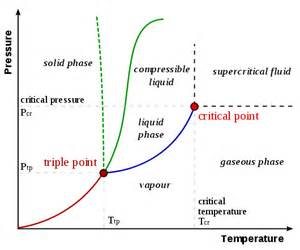
\includegraphics{MatterPhases.jpg}

At the phase boundaries, both states of matter can exist in phase equilibirum. \\
All three phases co-exist at the triple point \\
Beyond the critical point, you cannot define between liquid and gas \\
Dotted green line is for water

\section*{Phase Changes}
Phase changes occur at a unique temperature for set pressure, and use the latent heat specific to each transition:
\vspace{-8pt}
\begin{itemize}
    \item[] Between solid \& liquid: latent heat of fusion
    \item[] Between liquid \& gas: latent heat of vaporisation
    \item[] Between solid \& gas: latent heat of sublimation
\end{itemize}
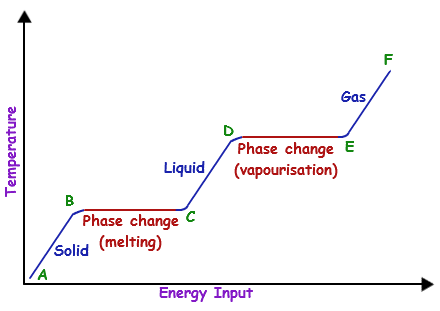
\includegraphics[scale=0.75]{download.png}

\section*{Calorimetry}
\begin{itemize}
    \item Calculations of energy transferred as heat to change temperature \& heat
    \item Heat is conserved for closed systems
    \item Chemical reactions analogous to phase changes e.g. heat of combustion
\end{itemize}

\section*{Applications of Phase Changes}
\begin{itemize}
    \item Steam-heating systems -- Victorian era stuff
    \item Temperature control
    \item Perspiration -- sweat cooling
\end{itemize}

\chapter{}
\section*{Recap}
Heat: energy transferred between bodies at different temperatures \\
Specific heat capacity: J mol\textsuperscript{-1} K\textsuperscript{-1} / J kg\textsuperscript{-1} K\textsuperscript{-1} \\
Phase changes and calorimetry

\section*{Learning Aims}
\begin{itemize}
    \item Thermal Expansion using original dimensions and temp. change of material
    \item Define thermal stress in terms of elastic properties
    \item Characteristics of 3 heat transfer mechanisms
    \item Define heat current in terms of thermal conductivity
    \item Stefan-Boltzmann Law -- Black Bodies
\end{itemize}

\section*{Thermal Expansion}
Used in thermometry \\
Implications for engineering -- rigid structures that are heated

Linear Thermal Expansion:
\vspace{-8pt}
\begin{itemize}
    \item Original rod length, L\textsubscript{0}
    \item Small change in temp, ${\Delta}T \rightarrow \text{change in length, } {\Delta}L$
\end{itemize}
\vspace{-8pt}
\begin{equation*}
    {\Delta}L = {\alpha}L_{0}{\Delta}T
\end{equation*}
$\alpha$ is the linear expansion co-efficient with units K\textsuperscript{-1}

Volume Expansion:\\
For small temperature, $\Delta$T, we have change $\Delta$V in volune:
\begin{equation*}
    {\Delta}V = {\beta}V_{0}{\Delta}T
\end{equation*}
$\beta$ is the co-efficient of volume expansion, $\text{K}^{-1}$

\section*{Relating ${\alpha}$ and ${\beta}$}
For a cube of dimension, L, with V = $\text{L}^{3}$
Consider infinitesimal changes dV, dL, \& dT:
\begin{equation*}
	dV = \dfrac{dV}{dL}dL = 3L^{2}~dL
\end{equation*}
For intial cube dimensions, L\textsubscript{0} and V\textsubscript{0}, with $V_{0} = L_{0}^{3}$
\begin{gather*}
	dL = {\alpha}L_{0}dT \\
	dV = 3L^{2}{\alpha}L_{0}dT = 3{\alpha}V_{0}dT \\
	{\Delta}V = {\beta}V_{0}{\Delta}T \\
	\beta = 3\alpha
\end{gather*}

\section*{Thermal Expansion of Water}
Expansion of water is approximately linear to temperature macroscopically \\
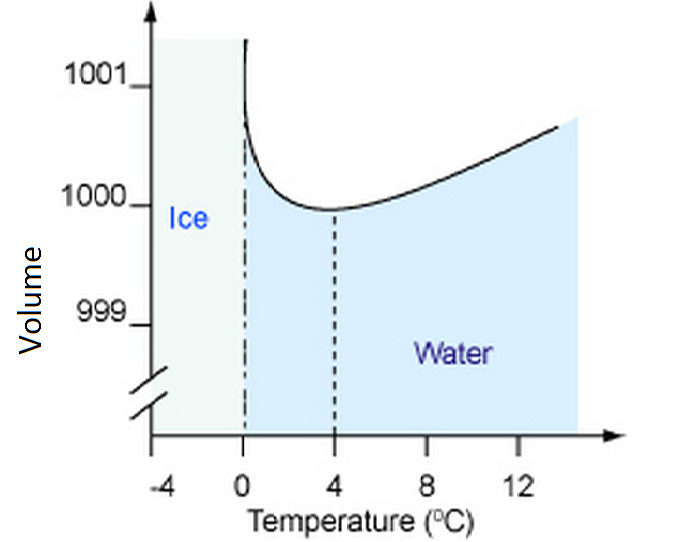
\includegraphics[scale=0.4]{water.png}

Water contracts as it cools down to 4{\textdegree}C, then expands. \\
This explains why ponds freeze from the top which was critical for evolution.

\section*{Thermally-Induced Stress}
Consider a material held in position such that the dimensions can't be changed\\
Now change temperature $\rightarrow$ stress is created
\begin{equation*}
	\text{Stress} = \frac{F}{A}
\end{equation*}
Young's modulus, Y -- Elastic behaviour of material:
\begin{equation*}
	Y = \frac{F}{A}\frac{L_{0}}{{\Delta}L} \text{ -- ratio of stress/strain}
\end{equation*}
For $L_{0}$, $(\frac{{\Delta}L}{L_{0}})_{thermal} = \alpha{\Delta}T$

When expansion is prevented: Using Young's modulus
\begin{gather*}
	\bigg(\frac{{\Delta}L}{L_{0}}\bigg)_{thermal} = \frac{F}{AY} \rightarrow \\
	\bigg(\frac{{\Delta}L}{L_{0}}\bigg)_{thermal} + \bigg(\frac{{\Delta}L}{L_{0}}\bigg)_{force} = \alpha{\Delta}T + \frac{F}{AY} = 0 \rightarrow \\
	\frac{F}{A} = -Y\alpha{\Delta}T
\end{gather*}

\section*{Heat Transfer Process}
Three mechanisms of heat transfer:
\vspace{-12pt}
\begin{itemize}
	\item convection -- motion of mass between regions
	\item conduction -- vibration through materials
	\item radiation -- electromagnetic radiation; no medium
\end{itemize}
\vspace{-8pt}
Conduction: \\
Heat flows from hot to cold \\
Energy dQ is transferred in time dt \\
Heat current $= H = \frac{dQ}{dt} \text{; }~~ H~\propto~A$ \\
Experimentally, $H = \frac{dQ}{dt} = kA\frac{T_{H}-T_{C}}{L}$, where $k$ is the thermal conductivity of the material in $W~m^{-1}~K^{-1}$

The general form for H, for non-uniform dT, is given by:
\begin{equation*}
	H = \frac{dQ}{dt} = -kA\frac{dT}{dx}\text{, negative sign indicates heat flows in direction of decreasing temperature}
\end{equation*}
Engineers use thermal resistance, $R = L/k \text{, in units of } K~m^{2}~W^{-1}$

Convection: \\
Convey heat energy from one location to another by movemnet of fluid (gas or liquid) with higher temperature. \\
Two types:
\vspace{-8pt}
\begin{itemize}
	\item Natural Convection e.g. hot air rising
	\item Forced Convection e.g. blood circulation
\end{itemize}
\vspace{-8pt}
This is from complex fluid dynamics processes and so, there are no simple models.

Radiation: \\
Through the electromagnetic spectrum so does not require a medium -- can go through vacuums
Radiation depends on body temperature -- hotter bodies emit shorter wavelengths of radiation
\begin{equation*}
	H = Ae{\sigma}T^{4}
\end{equation*}
Rate of heat loss proportional to A, emissivity, e, \& temperature \\
This is the Stefan-Boltzmann Law, where $\sigma = 5.67\times10^{-8}~W~m^{-2}~K^{-4}$

Net heat current is the sum of the energy out and in from the surroundings at a temperature, T\textsubscript{s}, \& an emissivity, e\textsubscript{s}:
\begin{equation*}
	H_{net} = Ae{\sigma}T^{4} - Ae_{s}{\sigma}T^{4}_{s}
\end{equation*}

\chapter{}
\section*{Recap}
Black body emissivity, $e = 1$ \\
$T_{peak} ~\propto~f_{rad}$ \\
Many astro-bodies are approximately black bodies

\section*{Learning Aims}
\begin{itemize}
	\item Define an ideal gas \& understand the equation of state
	\item How a real has differs from an ideal gas
	\item Particle interactions \& importance of potential wells
	\item Phase diagrams \& importance of the triple \& critical points
\end{itemize}

\section*{Equations of state}
The state of a material can be entirely described by a small number of variables \\
Gases are described by the relationship between p, V, T, \& n \\
All of this is combined into the equation of state

\section*{Ideal Gases}
For total mass, $m_{total}$, \& known molar mass then we get number of moles, $n$:
\begin{equation*}
	m_{total} = n \times \text{gfm}
\end{equation*}
Holding other variables constant: (For an ideal gas only)
\vspace{-8pt}
\begin{itemize}
	\item $V~\propto~n$
	\item $V~\propto~\frac{1}{p}$ -- Boyle's Law
	\item $V~\propto~T$ -- Charles' Law
\end{itemize}

\section*{Ideal Gas Law}
\vspace{-24pt}
\begin{equation*}
	pV = nRT
\end{equation*}
R is the universal gas constant, $R \approx 8.31 J mol^{-1} K^{-1}$

Applicability: works well for moderate pressures and temperatures -- typically around ambient temperatures and atmospheric pressures \\
Gas density:
\begin{align*}
	n = \frac{m}{\text{gfm}} ~~~\&~~~ \rho = \frac{M}{V} \implies \rho = \frac{p\times\text{gfm}}{RT}
\end{align*}
If there is constant mass or n, then nR is constant:
\begin{gather*}
	\frac{pV}{T} = nR \implies \frac{pV}{T} = k \\
	\therefore ~~\frac{p_{1}V_{1}}{T_{1}} = \frac{p_{2}V_{2}}{T_{2}}
\end{gather*}

\begin{tabular}{c|c}
	Ideal Gases & Real Gases \\
	\hline
	Molecules infinitely small & Molecules have volume \\
	Perfectly elastic collisions & Lose kinetic energy upon collisions \\
	Do no interact with each other & Exert forces on each other
\end{tabular}

\section*{Van der Waal's Equation}
\vspace{-22pt}
\begin{equation*}
	\Big(p+\frac{an^{2}}{V^{2}}\Big)(V-nb) = nRT
\end{equation*}
This accounts for particle volume and interactions. \\
b $\approx$ volume of one mole of the gas \\
a $\approx$ quantifies forces attracting molecules, reducing pressure

\section*{pV diagrams}
These are important for thermodynamic processes. \\
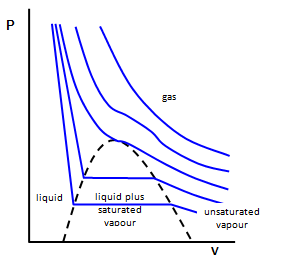
\includegraphics{pV.png} \\
Each line on a pV diagram indicates a fixed temperature -- higher temperatures are further from the axes \\
These lines of fixed temperature are called isotherms \\
For ideal gas, isotherms represent constant pV \\
Peak of dotted line shows critical temperature, above which there is no liquid-vapour phase transition \\
Below the critical temperature, gas condenses to liquid as it is compressed \\
Equilibrium between liquid and vapour phases inside dotted line region \\
The gas is never liquid above critical temperature; below critical temperature, gas changes state at constant p in phase equilibrium zone

\section*{Molcules \& Forces}
Molecules can vary massively in size \\
In gases, molecules are free to move; In liquids and solids, they are held together by intermolecular forces \\
Forces are electrical in origin -- attractional/repulsive \& $\propto \frac{1}{r^{2}}$, i.e. $U(r)\propto\int\! f(r)\; dr$

\section*{Force \& Potential Energy}
Molcules are not point charges -- they contain $+$ve \& $-$ve parts \\
Attractive interactions increase at distance up to $r_{0}$ then become repulsive. \\
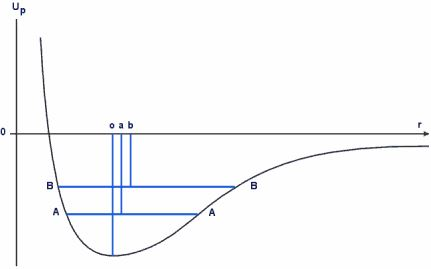
\includegraphics[scale=0.9]{PotWell.jpg} \\
Region near bottom of graph called a potential well -- potential $U_{o}$ at position o.
\begin{align*}
	E_{k} << |U_{o}| \text{ -- Solid};\quad
	E_{k} < |U_{o}| \text{ -- Liquid};\quad
	E_{k} > |U_{o}| \text{ -- Gas}
\end{align*}
As temperature increases, the phase changes and importance of kinetic energy increases

Thermal expansion -- molecular view:
As energy $\uparrow$, average distance $\uparrow$
Adding heat to a solid causes molecules to rise up the potential well \\
Atomic vibrations increase the radii defined by the sides of the well

\section*{Phase diagrams}
These are plots of p against T \\
There is only one phase at any specific p \& T, apart from phase boundaries where phase equilibrium occurs \\
Triple point -- there is no liquid phase for materials with a triple point pressure $>$ the given pressure \\
Critical point -- beyond this, as in latent heat, liquids and gases cannot be distinguished between, and are collectively called fluids

\chapter{}
\section*{Learning Aims}
\begin{itemize}
	\item Known assumptions of kinetic theory for ideal gases
	\item Demonstrate relation between pressure and molecular properties
	\item Translational kinetic energy
	\item RMS speed
	\item Mean free path
\end{itemize}

\section*{Kinetic Theory}
Model has as large number of molecules in a box \\
Assumptions made:
\vspace{-8pt}
\begin{itemize}
	\item[] Point particles
	\item[] There is a volume, V, from a large number, N, of molecules with mass, m
	\item[] Molecules are in constant motion, obeying Newton's law
	\item[] Perfectly elastic collisions
	\item[] Walls of box are perfectly rigid and infinitely massive (they do not absorb any energy)
\end{itemize}
\vspace{-8pt}
Molecular motion $\rightarrow$ pressure of system
\begin{equation*}
	F = \frac{mv-mu}{t} = \frac{dp}{dt}
\end{equation*}
Individual $\Delta$p for number, N, of particles \\
All molecules collide with walls -- generate pressure \\
Assume all have velocity, $v = |v_{x}|$
\begin{gather*}
	m|v_{x}| - (-m|v_{x}|) = 2m|v_{x}| \\
	\text{Wall Area, A, and number of molecules per unit volume, N/V} \\
	\text{No. of collisions at A in dt} = \frac{1}{2}\Big(\frac{N}{V}\Big)\big(A|v_{x}|dt\big)
\end{gather*}
Assume half of these are moving towards the wall:
\begin{gather*}
	{\Delta}p_{x}: dp_{x} = \frac{1}{2}\Big(\frac{N}{V}\Big)\big(A|v_{x}|dt\big) \times 2m|v_{x}| \\
	\implies \frac{NAmv^{2}_{x}dt}{V} \\
	\implies F = \frac{dp_{x}}{dt} = \frac{NAmv^{2}_{x}}{V} \\
	\implies p = \frac{F}{A} = \frac{Nmv^{2}_{x}}{V} \\
	\therefore pV = Nmv^{2}_{x} \\
	\implies pV = nRT
\end{gather*}

\section*{Average Velocities}
Assumed all molecules have $v_{x}$ \\
Replace this with $\bar{v}_{x}$ \\
Must have $v^{2} = v_{x}^{2} + v_{y}^{2} + v_{z}^{2},~ \bar{v} = \sum v_{x,y,z}$ \\
Overall, velocities must cancel out:
\begin{gather*}
	\bar{v}_{x}^{2} = \bar{v}_{y}^{2} = \bar{v}_{z}^{2} \\
	\bar{v}_{x}^{2} = \frac{1}{3}\bar{v}^{2} \\
	\therefore pV = \frac{1}{3}Nm\bar{v}^{2} \\
	\implies = \frac{2}{3}N(\frac{1}{2}m\bar{v}^{2}) \\
	\implies = \frac{2}{3}NE_{k} \text{, for translational }E_{k}
\end{gather*}
Total translational kinetic energy labelled $K_{tr}$
\begin{gather*}
	\bar{K}_{tr} = \frac{1}{2}m\bar{v}^{2};~~ \sum N \rightarrow \text{total }K_{tr} \\
	pV = \frac{2}{3}K_{tr} = nRT \text{ (whole gas)} \\
	\implies K_{tr} = \frac{3}{2}nRT\text{, for n moles of gas} \\
	\text{Divide }K_{tr}\text{ by N to get per molecule} \\
	\frac{K_{tr}}{N} = \frac{1}{2}m\bar{v}^{2} = \frac{3nRT}{2N} \\
	\implies = \frac{3}{2}\Big(\frac{R}{A}\Big)T ~\because~ \frac{n}{N} = \frac{1}{A} \\
	\bar{K}_{tr} = \frac{1}{2}m\bar{v}^{2} = \frac{3}{2}k_{B}T ~\because~ \frac{R}{A} = k_{B}\text{, the Boltzmann constant} \\
	pV = Nk_{B}T
\end{gather*}
\section*{RMS Speed}
RMS Speed stands for "Root Mean Square" speed:
\begin{gather*}
	v_{rms} := \sqrt{\bar{(v^{2})}} \\
	v_{rms} = \sqrt{\frac{3k_{B}T}{m}}\text{, for molecules} \\
	v_{rms} = \sqrt{\frac{3RT}{M}}\text{, for the whole gas}
\end{gather*}
RMS speed is greater than average speed \\
RMS speed is greater for molecules with smaller masses

\section*{Collisions}
Consider N spherical molecules of radius, r, with volume, V \\
Molecules sweep out cylinder of radius 2r as they go -- inside this cylinder, collisions will occur \\
In an interval dt, molecules travel v{\,}dt \\
For dN molecules with cylinder:
\begin{gather*}
	dN = 4{\pi}r^{2}vdt\Big(\frac{N}{V}\Big) \\
	\text{Collision Rate: } \frac{dN}{dt} = \frac{4{\pi}r^{2}vN}{V}
\end{gather*}
If all particles are moving, a factor of $\sqrt{2}$ is needed:
\begin{equation*}
	\frac{dN}{dt} = \frac{4\sqrt{2}{\pi}r^{2}vN}{V}
\end{equation*}

\section*{Mean free path, $\lambda$}
We take the reciprocal of above to get time:
\begin{gather*}
	\frac{dN}{dt} = \frac{4\sqrt{2}{\pi}r^{2}vN}{V} \rightarrow \frac{dt}{dN} = \frac{V}{4\sqrt{2}{\pi}r^{2}vN} \\
	\implies \bar{t} = \frac{V}{4\sqrt{2}{\pi}r^{2}vN} ~\because~ dN = 1 \\
	\lambda = v\bar{t} = \frac{V}{4\sqrt{2}{\pi}r^{2}N}
\end{gather*}
This can be desrcibed macroscopically by using $pV = Nk_{B}T$:
\begin{equation*}
	\lambda = \frac{k_{B}T}{4\sqrt{2}{\pi}r^{2}p}
\end{equation*}

\chapter{}
\section*{Learning Aims}
\begin{itemize}
	\item Heat capacity of monatomic gas
	\item Equipartition principle
	\item Degrees of freedom \& heat capacities of gases
	\item Dulong \& Petit rule from equipartition principle
	\item Degrees of freedom reduce at low temperature
	\item Distribution function in terms of molecular speed
	\item Maxwell-Boltzmann distribution
\end{itemize}
\section*{Heat capacities}
Heat is energy in transit -- adding heat adds energy \\
Kinetic energy $\propto$ temperature, for ideal gases \\
Equipartition theory -- energy on average is shared equally across all available Degrees of Freedom (DoFs) \\
For a simple atomic gas -- there are 3 axes of translational motion $\therefore$ 3 DoFs \\
Raising energy raises temperature

How much heat is needed? \\
\textit{dQ $\rightarrow$ dT relates to change in kinetic energy, $dK_{tr}$}\\
Define $C_{V}$ to be molar heat capacity at constant volume:
\begin{gather*}
	dQ = dK_{tr} = \frac{3}{2}nRdT \\
	dQ = nC_{V}dT \\
	\therefore C_{V} = \frac{1}{n}\frac{dQ}{dT} = \frac{1}{n}\frac{dK_{tr}}{dT} \\
	\implies = \frac{1}{n}\frac{3nRdT}{2dT} \\
	\therefore C_{V} = \frac{3}{2}R
\end{gather*}

\section*{Degrees of Freedom}
There are two additional DoFs in diatomic molecules \\
Travelling along each dimensional axis, rotating about each axis, and vibrating through bonds all provide a DoF \\
Monatomic gas -- heat only goes into translational DoFs \\
For other molecules -- heat is distributed over all DoFs \\
Energy, on average, is spread equally between different types of motion \\
Each molecule carries averge energy of $\frac{1}{2}k_{B}T$ per DoF \\
Monatomic -- 3 DoFs from each translational dimension $\therefore \frac{3}{2}nRT \rightarrow C_{V} = \frac{3}{2}R$ \\
Diatomic -- 5 DoFs from 3 translational and 2 rotational $\therefore \frac{5}{2}nRT \rightarrow C_{V} = \frac{5}{2}R$ \\
There are quanitised energy levels in vibrational DoFs \\
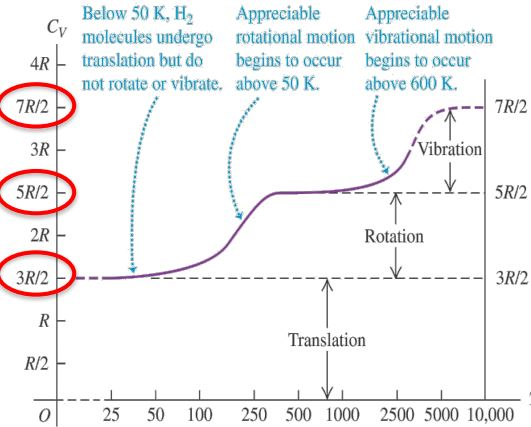
\includegraphics[scale=0.8]{Vibration.jpg} \\
Motions are "frozen out" at lower temperatures; as temperature increases, more DoFs become available

\section*{Dulong \& Petit Rule}
Consider the crystalline lattice of a solid \\
Each bond is under SHM -- x,y,z motion \\
Stretching of bonds stored potential energy in each axis

Dulong \& Petit Rule $\approx 25 J mol^{-1} K^{-1} \approx 3R$ for solids \\
For a simple spring model: there are 6 DoFs; 3 translational, 3 vibrational potential:
\begin{gather*}
	\text{Average energy per molecule } = \frac{6}{2}k_{B}T = 3k_{B}T = 3R \\
	\text{Over whole solid: } E_{total} = 3Nk_{B}T = 3nRT
	\therefore \text{Molar heat capacity, } C_{V} = 3R
\end{gather*}

\section*{Molecular Speeds}
Use a speed distribution function to map out molecular speeds:\\
Each plot has the same area \\
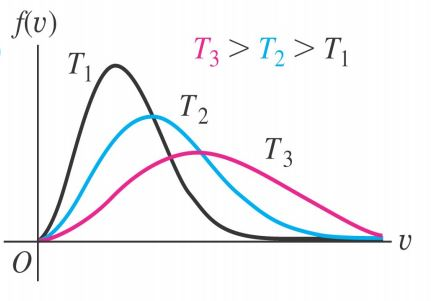
\includegraphics[scale=0.85]{Distribution.jpg}
\begin{gather*}
	\text{The number of molecules with set speeds: } dN = Nf(v)~dv \\
	\text{The probabaility that a molecule has a speed: } f(v)~dv
\end{gather*}
3 key values for molceular speeds:
\vspace{-8pt}
\begin{itemize}
	\item most probable; $v_{mp}$, where $\frac{df}{dv} = 0$
	\item average; $v_{av} = \int_{0}^{\infty} vf(v)~dv$
	\item rms; $v_{rms} = \sqrt{\bar{(v^{2})}} = \sqrt{\int_{0}^{\infty} v^{2}f(v)~dv}$
\end{itemize}
$f(v)$ is described by the Maxwell-Boltzmann distribution:
\begin{equation*}
	f(v) = 4{\pi}\bigg(\frac{m}{2{\pi}k_{B}T}\bigg)^{3/2}v^{2}e^{\frac{-mv^{2}}{2k_{B}T}}
\end{equation*}
Substituting this $f(v)$ into previous speed equations gives:
\begin{gather*}
	v_{mp} = \sqrt{\frac{2k_{B}T}{m}};~~~\bar{v} = \sqrt{\frac{8k_{B}T}{{\pi}m}};~~~v_{rms} = \sqrt{\frac{3k_{B}T}{m}}
\end{gather*}

\chapter{}
\section*{Learning Aims}
\begin{itemize}
	\item The First Law of Thermodynamics
\end{itemize}

\section*{Thermodynamic Systems}
Definition: A collection of objects regarded as a single unit $\rightarrow$ beyond those objects is classified as the surroundings

Heat, Q, can flow \emph{in to} or \emph{out of} a system \\
Work, W, can br \emph{done by} or \emph{done on} a system \\
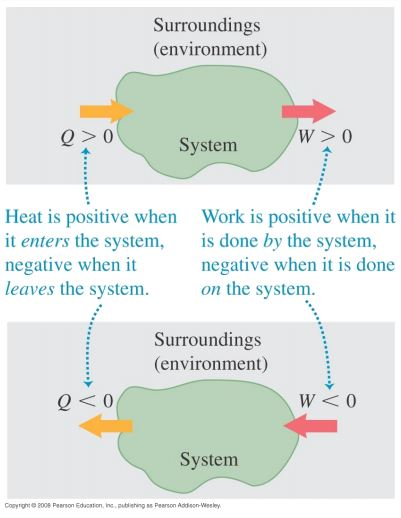
\includegraphics{ThermoSystem.jpg} \\
Consider gas in a piston:
Molecules hit piston, transfer energy as piston moves out $\rightarrow$ lower kinetic energy so lower temperature
\begin{equation*}
	\text{Work } dW = F\:dx
\end{equation*}
Piston pushes molecules, transfers energy as piston moves in $\rightarrow$ higher kinetic energy so higher temperature
\begin{gather*}
	F = pA \rightarrow dW = F\;dx = pA\:dx \\
	A\:dx = dV \rightarrow dW = p\:dV \\
	\implies W = \int_{V_{1}}^{V_{2}} p\:dV \text{ -- [Integrate over volume change]}
\end{gather*}
However, pressure depends on volume and temperature \\
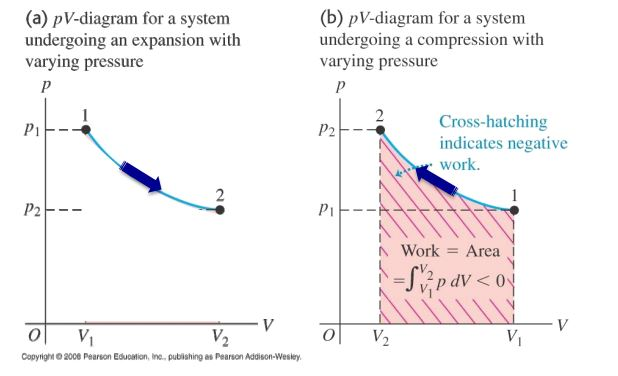
\includegraphics[scale=0.8]{pV.jpg} \\
Work is the area under the curve
\begin{gather*}
	p_{1}V_{1} = nRT_{H}; \; p_{2}V_{2} = nRT_{H} \\
	p_{2} = 2p_{1} \therefore V_{2} = \frac{V_{1}}{2} \\
	\implies W = \int_{V_{1}}^{V_{2}} p\:dV = \int_{V_{1}}^{V_{2}} \frac{nRT_{H}}{V}\:dV \\
	\implies = nRT_{H}[\ln{V}]_{V_{1}}^{V_{2}} = nRT_{H}\ln{\frac{V_{2}}{V_{1}}} \\
	\therefore W = -nRT_{H}\ln{2}
\end{gather*}
Work is path-dependent: different routes from initial to final volumes and pressures will require a different amount of work -- due to work being the area under the graph \\
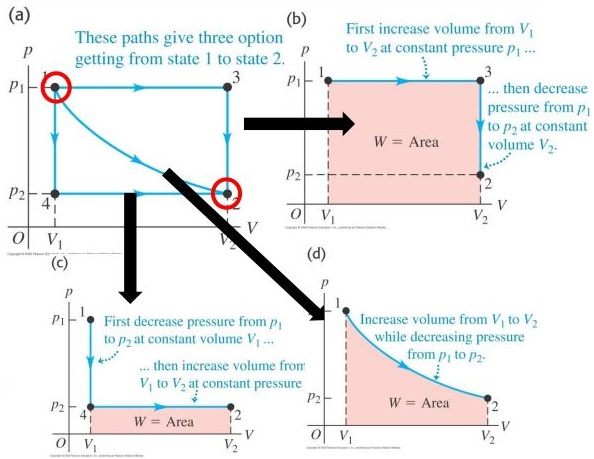
\includegraphics[scale=0.8]{Paths.jpg} \\
(c) takes the least work as it has the smallest area

\section*{First Law of Thermodynamics}
Internal energy, U -- sum of all $E_{k}$ and $E_{p}$ in a system (not gravitational potential though)
\begin{gather*}
	{\Delta}U = U_{2} - U_{1} \\
	+ Q, \uparrow U \rightarrow {\Delta}U = Q \\
	\text{Work done uses internal energy: } W = -{\Delta}U
\end{gather*}
The first law of thermodynamics is stated as:
\begin{gather*}
	U_{2} - U_{1} = {\Delta}U = Q - W \quad \text{OR: } Q = {\Delta}U + W; \; dU = dQ - dW
\end{gather*}
Absolute U is difficult to measure for a system; $\Delta$U is not \\
Experimentally: Q \& W depend on path taken but \underline{$\Delta$U is independent of path}

\section*{Special Case 1}
Isolated system -- no work or heat is interchanged with surroundings: $W = Q = 0$ \\
U is constant, only depends on T

\section*{Special Case 2}
Cyclic process -- a system that returns to intial state: $U_{2} = U_{1}$ \& $Q = W \therefore$ U is constant overall

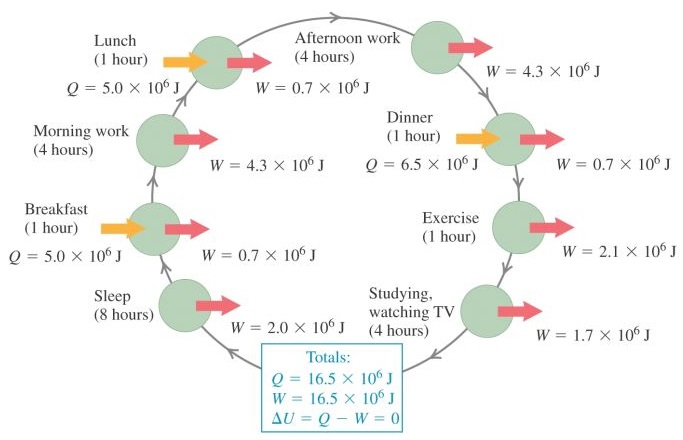
\includegraphics[scale=0.9]{Cyclic.jpg}

\chapter{}
\section*{Recap}
For ideal gases: $E_{T} = K_{tr} = \frac{3}{2}RT$ (per mole?) \\
For real gases: $E_{T} = K_{tr} + E_{P} = \frac{3}{2}RT - \frac{a}{V}$ (per mole?) \\
Free expansion causes decrease in temperature -- reason for extra term in real gases

\section*{Learning Aims}
\begin{itemize}
	\item Four thermodynamic process
	\item Ideal gases \&  different molar heat capacities for constant volume \& pressure
	\item Derive relationship between these heat capacities
	\item Derive relationship for adiabatic process
\end{itemize}

\section*{Thermodynamic Processes}
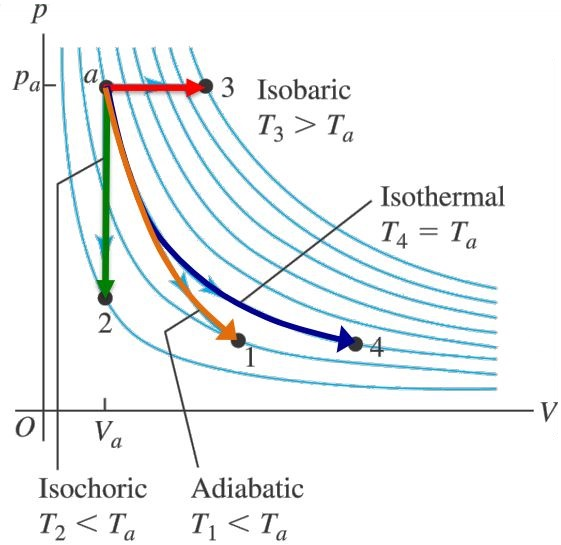
\includegraphics[scale=0.7]{Processes.jpg} \\
For an ideal gas:
\vspace{-8pt}
\begin{itemize}
	\item[] Isobaric process, ${\Delta}p = 0$
	\item[] Isochoric process, ${\Delta}V = 0 \rightarrow W = 0$
	\item[] Isothermal process, ${\Delta}T = 0$
	\item[] Adiabatic process, $Q = 0$
\end{itemize}

\section*{Isobaric Processes}
Constant pressure process:
\begin{equation*}
	W = p(V_{2} - V_{1})
\end{equation*}

\section*{Isochoric Processes}
Constant volume process:
\begin{gather*}
	{\Delta}V = 0 \therefore W = 0 \\
	\implies p\:dV = 0 \\
	U_{2} - U_{1} = {\Delta}U = Q
\end{gather*}
All energy added to the system as heat goes into raising the internal energy

\section*{Isothermal Processes}
Constant temperature process: \\
Heat flow must occur slowly enough that thermal equilibrium is maintained \\
Generally -- W, Q, \& ${\Delta}U \neq 0$ \\
Ideal gas -- ${\Delta}U = 0$, $Q = W$

i.e. All heat energy taken in is output as work done

\section*{Adiabatic Processes}
No heat transfer process:
\vspace{-10pt}
\begin{equation*}
	Q = 0 \therefore U_{2} - U_{1} = {\Delta}U = -W
\end{equation*}
Occurences:
\vspace{-8pt}
\begin{enumerate}
	\item System is well-insulated
	\item Process was so quick that heat flow was neglected
\end{enumerate}
\vspace{-8pt}
For ideal gases in expansion, W is positive so $\Delta$U drops $\rightarrow$ temperature drops

\section*{Heat Capacity}
Two molar heat capacities:
\vspace{-8pt}
\begin{itemize}
	\item[] At constant volume, $C_{V}$
	\item[] At constant pressure, $C_{p}$
\end{itemize}
\vspace{-8pt}
For ideal gases, $C_{p} > C_{V}$

Consider n moles of gas at temperature T in constant volume, V \\
Add heat, dQ:
\begin{gather*}
	dQ = nC_{V}dT \implies dU = nC_{V}dT \because W = 0 \\
	\text{Now at constant pressure: } dQ = nC_{p}dT
\end{gather*}
Material expands when heated so from ideal gas law:
\begin{gather*}
	dW = p\:dV = nR\:dT
\end{gather*}
Using the first law of thermodynamics:
\begin{gather*}
	dQ = dU + dW \\
	\implies nC_{p}dT = nC_{V}dT + nRdT \\
	\implies C_{p} = C_{V} + R ~\because~ dT \text{ is the same}
\end{gather*}

\section*{Ratio of heat capacities}
\vspace{-22pt}
\begin{equation*}
	\gamma = \frac{C_{p}}{C_{V}}
\end{equation*}
For a monatomic gas, $\gamma \approx 1.67$ \\
For a diatomic gas, $\gamma = 1.4$

\section*{The Adiabatic Process}
An adiabatic curve at any point is always steeper than the isotherm passing through the same point. \\
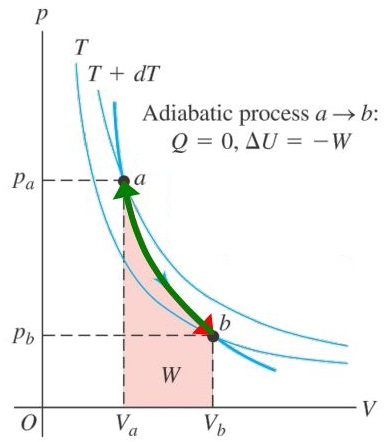
\includegraphics[scale=0.7]{Adiabatic.jpg} \\
Idealised process so one of two cases:
\vspace{-8pt}
\begin{enumerate}
	\item Really fast process -- no heat is exchanged
	\item Really slow process -- Thermal Equilibrium is maintained
\end{enumerate}
\vspace{-8pt}
For an ideal gas: temperature drops for expansion and rises for compression

\section*{Relating V, T, p, \& W}
\vspace{-24pt}
\begin{gather*}
	dU = -dW \text{ [infinitesimal process]} \\
	\implies nC_{V}dT = -pdV ~\&~ pV = nRT \\
	\implies nC_{V}dT = -\frac{nRT}{V}\:dV \\
	\implies \frac{dT}{T} + \frac{R}{C_{V}}\frac{dV}{V} = 0 ~\&~ \gamma = \frac{C_{p}}{C_{V}} \\
	\implies \frac{R}{C_{V}} = \frac{C_{p} - C_{V}}{C_{V}} = \frac{C_{p}}{C_{V}} - 1 = \gamma - 1
\end{gather*}
Now take last equation and integrate:
\begin{gather*}
	\int \bigg[\frac{dT}{T} + (\gamma - 1)\frac{dV}{V} = 0\bigg] \\
	\implies \ln{T} + (\gamma - 1)\ln{V} = k \\
	\implies \ln{T} + \ln{V^{\gamma - 1}} = k \\
	\implies \ln{TV^{\gamma - 1}} = k \\
	\implies TV^{\gamma - 1} = \kappa
\end{gather*}
Hence, for initial and final states, ($T_{1},\:V_{1}$) \& ($T_{2},\:V_{2}$):
\begin{gather*}
	T_{1}V_{1}^{\gamma - 1} = T_{2}V_{2}^{\gamma - 1} ~\&~ T = \frac{pV}{nR} \\
	\therefore p_{1}V_{1}^{\gamma} = p_{2}V_{\gamma}
\end{gather*}
Now considering work:
\begin{gather*}
	Q = 0 ~\therefore~ W = -{\Delta}U ~\&~ {\Delta}U = nC_{V}{\Delta}T \text{ for ideal gases} \\
	W = nC_{V}(T_{1} - T_{2}) \\
	pV = nRT \rightarrow W = \frac{C_{V}}{R}(p_{1}V_{1} - p_{2}V_{2}) \\
	\implies W = \frac{1}{\gamma - 1}(p_{1}V_{1} - p_{2}V_{2})
\end{gather*}

\chapter{}
\section*{Learning Aims}
\begin{itemize}
	\item Principles of a heat engine \& its thermal efficiency
	\item Sketch the Otto cycle, desrcibe each step, \& understand its limitations
	\item Describe differences between Otto cycle \& the diesel engine
	\item How a fridge works \& derive the coefficient of performance
\end{itemize}

\section*{Definitions}
A device that converts heat into mechanical energy of work is known as a heat engine

Matter inside this engine undergoes thermodynamic processes -- \emph{the working substance}

The simplest engines are thosein which the working substance undergoes a cyclic process

\section*{A Simple Heat Engine}
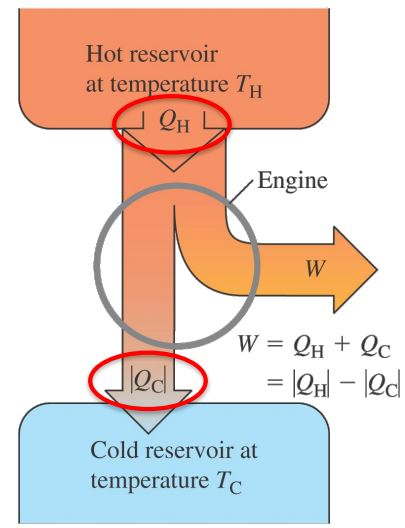
\includegraphics[scale=0.7]{HeatEngine.jpg} \\
All heat engines absorb heat from the hot reservoir \& discard it to the cold reservoir \\
Energy from the hot reservoir, $Q_{H}$, is positive; energy lost to cold reservoir, $Q_{C}$, is negative \\
The energy difference is the work done, W

\section*{Efficiency}
$Q_{H}$ and $Q_{C}$ are the heat energies absorbed and rejected in one cycle of the heat engine -- the difference is the Work done
\begin{equation*}
	W = {\Delta}Q = Q_{H} + Q_{C} = |Q_{H}| - |Q_{C}|
\end{equation*}
Thermal efficiency, e:
\begin{equation*}
	e = \frac{W}{Q_{H}} = 1 + \frac{Q_{C}}{Q_{H}} = 1 - \bigg|\frac{Q_{C}}{Q_{H}}\bigg|
\end{equation*}
A heat engine can never be 100\% efficient $\rightarrow e < 1$ \\
If $|Q_{C}| = 0$, then there can be no heat flow so no work can be undertaken

\section*{The Otto Cycle}
The Otto Cycle is an idealised model for an internal combustion engine \\
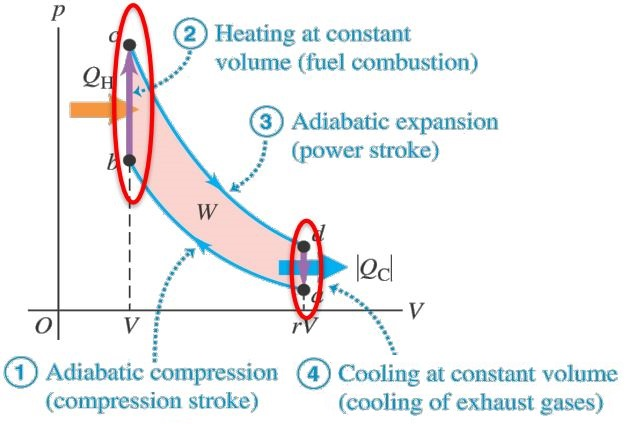
\includegraphics[scale=0.8]{Otto.jpg} \\
The maximum volume of the cylinder is a factor, \emph{r} -- the compression ratio, larger than the minimum volume: $V_{max} = rV_{min}$ \\
$Q_{H} > Q_{C} \therefore$ Work is done

bc \& da are at constant volume so:
\begin{gather*}
	Q_{H} = nC_{V}(T_{c} - T_{b}) > 0 ~\&~ Q_{C} = nC_{V}(T_{a} - T_{d}) < 0 \\
	\implies e = \frac{Q_{H} + Q_{C}}{Q_{H}} = \frac{T_{c} - T_{b} + T_{a} - T_{d}}{T_{c} - T_{b}}
\end{gather*}
For ab and cd:
\begin{gather*}
	T_{a}(rV)^{\gamma - 1} = T_{b}V^{\gamma - 1} ~\&~ T_{d}(rV)^{\gamma - 1} = T_{c}V^{\gamma - 1} \implies e \\
	e = \frac{T_{d}r^{\gamma - 1} - T_{a}r^{\gamma - 1} + T_{a} - T_{d}}{T_{d}r^{\gamma - 1} - T_{a}r^{\gamma - 1}} = \frac{(T_{d} - T_{a})(r^{\gamma - 1} - 1)}{(T_{d} - T_{a})r^{\gamma - 1}} \\
	e = 1 - \frac{1}{r^{\gamma - 1}} \\
	\therefore ~ e < 1 \emph{always}
\end{gather*}
e.g. for air: $\gamma = 1.4, ~ r = 8 \implies e \approx 0.56$ \\
\emph{r} cannot be increased too mch as the temperature of adiabatic compression rises too high \& the air/fuel mixture ignites early -- 'knocking'

In reality, the Otto cycle neglects many other sources of energy loss e.g. friction, turbulence, incomplete combustion etc. \\
This leads to further inefficiences so in example above, $e \approx 0.35$ in reality

 \section*{The Diesel Cycle}
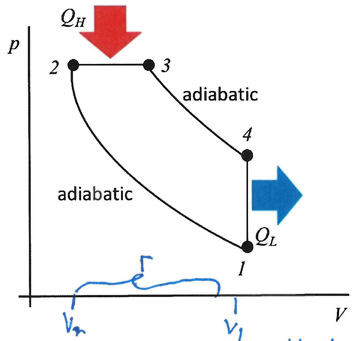
\includegraphics[scale=0.8]{Diesel.jpg}\\
Differences to the Otto Cycle:
\vspace{-8pt}
\begin{itemize}
	\item No spark plugs -- high temperature caused by adiabatic compression is used to ignite fuel at constant pressure
	\item Fuel is injected after compression -- no early ignition can occur
	\item Can have bigger \emph{r} (15-20)
	\item More efficient -- $e \approx 0.7$, ideally
\end{itemize}

\section*{Fridges}
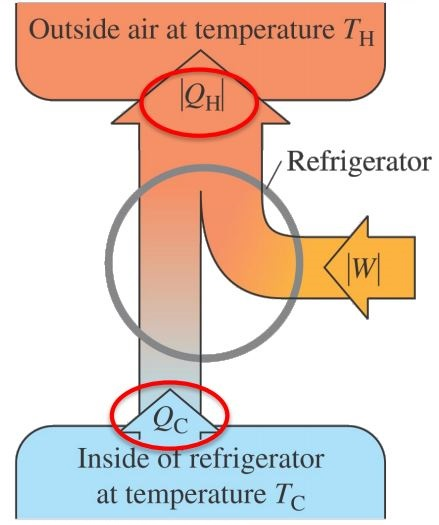
\includegraphics[scale=0.7]{Fridge.jpg} \\
Fridges can be considered a heat engine in reverse \\
Requires net input of work to drive extraction of heat from cold to hot \\
In this case, $Q_{C}$ is positive, and $Q_{H}$ \& W are negative (negative work is done on the system)

\section*{Co-efficient of Performance}
For a cyclic process, from the first law:
\begin{gather*}
	Q_{H} + Q_{C} - W = 0 ~\text{or}~ -Q_{H} = Q_{C} - W \\
	Q_{H} ~\&~ W < 0 \implies |Q_{H}| = Q_{C} + |W|
\end{gather*}
The best fridge removes the most heat for the least work -- evaluated by the coefficient of performance, \emph{K}:
\begin{equation*}
	K = \frac{Q_{C}}{W} = \frac{|Q_{C}|}{|Q_{H}| - |Q_{C}|}
\end{equation*}
Air conditioners use the same principle: for heat current H, input power P, \& time t:
\begin{equation*}
	K = \frac{|Q_{C}|}{|W|} = \frac{Ht}{Pt} = \frac{H}{P}
\end{equation*}
It is impossible to have a fridge without some input of work \\
A heat pump functions as an inside-out firdge: it takes heat from cold outside air to heat the inside

\chapter{}
\section*{Learning Aims}
\begin{itemize}
	\item Reversible \& irreversible processes
	\item Directionality of irreversible processes leads to the second law of thermodynamics and entropy
	\item Processes that form the Carnot Cycle \& its efficiency
	\item Importance of the Carnot Cycle as a heat engine \& temperature measurement
\end{itemize}

\section*{Direction of Processes}
The key to the second law of thermodynamic processes is the direction of thermodynamic processes \\
Real-life processes only proceed in one direction: Heat moves from hot to cold and cannot spontaneously reverse

It is possible to have idealised processes that are reversible -- these can only occur close to equilibrium (known as \emph{quasi-equilibrium}) \\
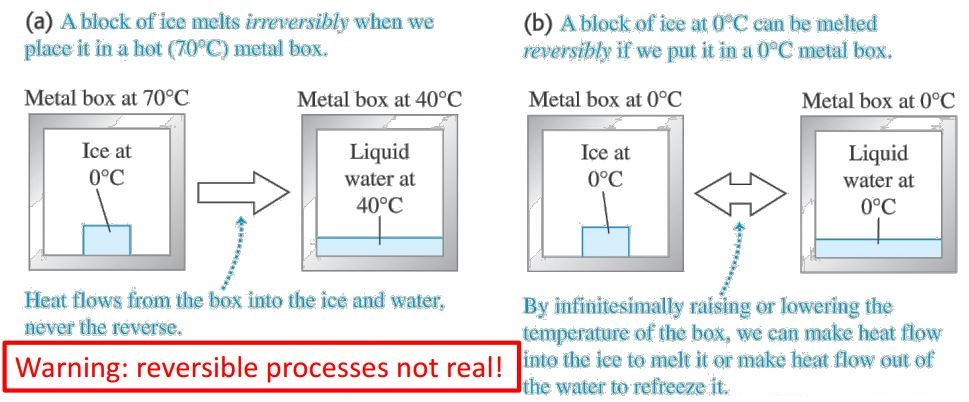
\includegraphics[scale=0.65]{Icebox.jpg}

\section*{The Second Law of Thermodynamics}
Kelvin-Planck statement on engines: \\
\emph{"It is impossible for any system to undergo a process in which it absorbs heat from a reservoir at a single temperature and converts the heat completely into mechanical work, with the system ending in the same state in which is began."}

Restating the Second law -- the Clausius statement on fridges: \\
\emph{"It is impossible for any process to have as its sole result the transfer of heat from a cooler body to a hotter one."}

If one form of the law is violated, then it can be used to violate the other form as well \\
There is no observational test for either expression of the law -- it is accepted as an axiom \\
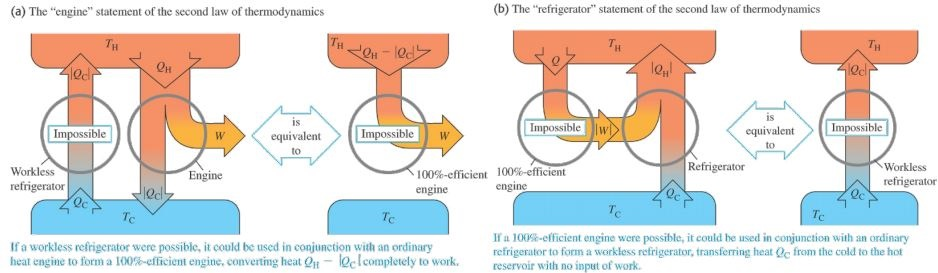
\includegraphics[scale=0.69]{Impossible.jpg} \\
Consider a moving body of molecules:
\vspace{-8pt}
\begin{itemize}
	\item[] Molecules have random motion; KE \& PE linked to internal energy
	\item[] Superimposed is a coordinated motion -- macroscopic motion \& KE
\end{itemize}
\vspace{-8pt}
Friction converts this macroscopic KE to random molecule motion but cannot fully convert random motion back into ordered macroscopic motion \\
THe direction of motion is linked to the \emph{degree of disorder}

\section*{The First Law vs The Second Law}
Certain processes are allowed by the First Law (energy conservation) but not by the Second Law (direction of processes) \\
e.g. powering a speedboat by extracting heat energy from the sea

The Second Law is a separate law of nature; it is not derived from the First Law

First Law: Energy cannot be created or destroyed \\
Second Law: The availability of useful energy is limited

\section*{The Carnot Cycle}
A hypothetical, idealised engine with maximum efficiency \\
This is consistent with the Second Law \\
Runs entirely on reversible processes:
\vspace{-8pt}
\begin{itemize}
	\item Isothermal heat transfers -- to avoid irreversible heat flow
	\item Adiabatic temperature changes -- to avoid irreversible heat transfer
	\item Thermal \& mechanical equilibrium must be maintined
\end{itemize}
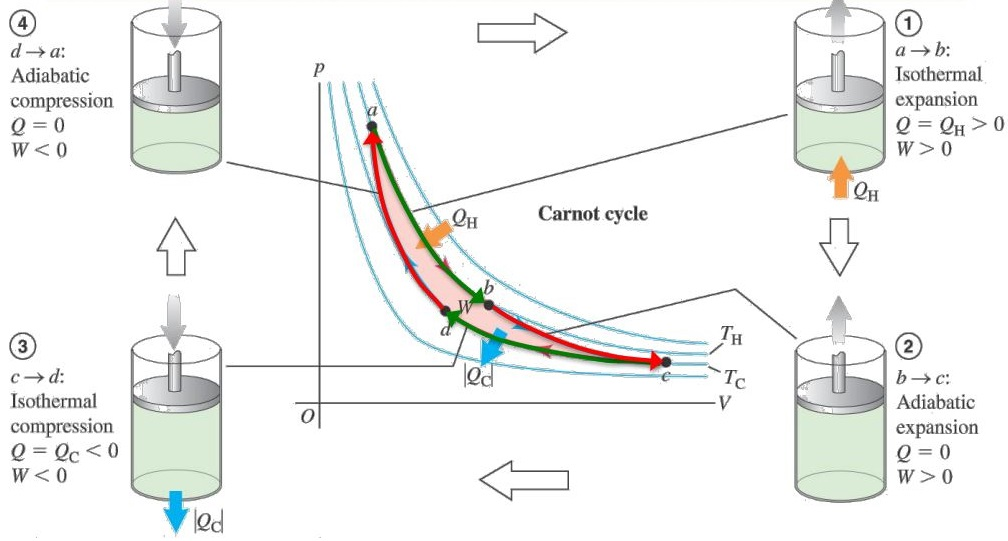
\includegraphics[scale=0.55]{Carnot.jpg}

\section*{Carnot Efficiency}
ab \& cd are isothermal so ${\Delta}U = 0$:
\begin{gather*}
	Q_{H} = W_{ab} = nRT_{H}\ln{\frac{V_{b}}{V_{a}}} ~\&~ Q_{C} = -nRT_{H}\ln{\frac{V_{c}}{V_{b}}} \\
	\implies \frac{Q_{C}}{Q_{H}} = -\frac{T_{C}}{T_{H}}\frac{\ln{(V_{c}/V_{d})}}{\ln{(V_{b}/V_{a})}}
\end{gather*}
bc \& da are adiabatic so:
\begin{gather*}
	T_{H}V_{b}^{\gamma - 1} = T_{C}V_{c}^{\gamma - 1} ~\&~ T_{H}V_{a}^{\gamma - 1} = T_{C}V_{d}^{\gamma - 1} \\
	\implies \frac{V_{b}^{\gamma - 1}}{V_{a}^{\gamma - 1}} = \frac{V_{c}^{\gamma - 1}}{V_{d}^{\gamma - 1}} ~\therefore~ \frac{V_{b}}{V_{a}} = \frac{V_{c}}{V_{d}}
\end{gather*}
This means that the logarithms in the isothermal equation are equal, and therefore cancel:
\begin{gather*}
	\frac{Q_{C}}{Q_{H}} = -\frac{T_{C}}{T_{H}} \implies \frac{|Q_{C}|}{|Q_{H}|} = \frac{T_{C}}{T_{H}}
\end{gather*}
The efficiency of the Carnot engine is therefore given by:
\begin{equation*}
	e_{Carnot} = 1 - \frac{T_{C}}{T_{H}} = \frac{T_{H} - T_{C}}{T_{H}}
\end{equation*}
Therefore, the larger the temperature difference, the more efficient the Carnot engine

\section*{Carnot Fridge}
Since all steps in the Carnot Cycle are reversible, the entire cycle may be run backwards to create a maximally efficient fridge \\
From the coefficient of performance \& the previous Carnot analysis:
\begin{gather*}
	K = \frac{|Q_{C}|}{|Q_{H}| - |Q_{C}|} = \frac{|Q_{C}|/|Q_{H}|}{1 - |Q_{C}|/|Q_{H}|} ~\&~ \frac{|Q_{C}|}{|Q_{H}|} = \frac{T_{C}}{T_{H}} \\
	\implies K_{Carnot} = \frac{T_{C}}{T_{H} - T_{C}}
\end{gather*}

\section*{Carnot Cycle and the Second Law}
No engine or fridge is more efficient than the Carnot cycle \\
All Carnot engines operating between the same two temperatures have the same efficiency, irrespective of the nature of the working substance \\
The Carnot efficiency sets the upper limit for real engines so $T_{H}$ is always maximised in practice

\section*{The Kelvin Scale}
As the Carnot Cycle efficiency is independent of the working substance, Kelvin proposed to use this to define his temperature scale as follows:
\begin{equation*}
	\frac{T_{C}}{T_{H}} = \frac{|Q_{C}|}{|Q_{H}|} = -\frac{Q_{C}}{Q_{H}}
\end{equation*}
Uses the triple point of water at 273.16 K to set the scale so identical to ideal has scale \\
Absolute zero is minimum (not zero) energy of a system -- leads to the Third Law of Thermodynamics

\chapter{}
\section*{Learning Aims}
\begin{itemize}
	\item Entropy \& entropy change for a reversible process
	\item Understand relationship between changes in entropy \& changes between states
	\item State the Second Law in terms of entropy
	\item Difference between macroscopic \& microscopic state descriptions
	\item Understand the Second Law in terms of microscopic state probabilities
\end{itemize}
\section*{Entropy}
The Second Law appears unlike other laws:
\vspace{-8pt}
\begin{itemize}
	\item Series of statements of impossibility
	\item Not a quantitive relationship
\end{itemize}
\vspace{-8pt}
However, it can be made quantitive by introducing concept of \underline{Entropy}: entropy is a measure of disorder

\section*{Defining entropy}
Consider a reversible infinitesimal isothermal expansion of ideal gas:
\begin{equation*}
	{\Delta}U = 0 \implies dQ = dW = p\:dV = \frac{nRT}{V}\:dV \implies \frac{dV}{V} = \frac{dQ}{nRT}
\end{equation*}
Expansion $\rightarrow$ molecules into a larger volume -- more disordered so $\frac{dV}{V}$ is a measure of increase in disorder \\
Denot entropy as \emph{S} and infinitesimal change \emph{dS}:
\begin{equation*}
	dS = \frac{dQ}{T} \implies {\Delta}S = \frac{{\Delta}Q}{T} \text{, for whole process}
\end{equation*}
Generalise any reversible process from state 1 to state 2 $\rightarrow$ as a series of infinitesimal steps at temperature, T:
\begin{equation*}
	{\Delta}S = \int_{1}^{2} \frac{dQ}{T}
\end{equation*}
Entropy is a function of the state of the system i.e. is independent of the path between the two states \\
This is similar to internal energy which is also state-, not path-dependent \\
Also similar to U, it is trivial to calculate changes in entropy $\Delta$S, but not absolute value of entropy, S \\
For reversible, cyclic processes, ${\Delta}S = 0$

\section*{Entropy in Irreversible Processes}
Since $\Delta$S is independent of path -- can model any change of state as a series of reversible processes so the previous equation can be used to calculate entropy change for irreversible processes too \\
All irreversible processes lead to an increase in entropy \\
Unlike energy, entropy is not a conserved quantity \\
Overall, Reversible cycles have ${\Delta}S = 0$; Irreversible processes always have positive $\Delta$S
It is possible to calculate $\Delta$S fpr free expansion by considering the isothermal path:
\begin{figure}[H]
	\begin{subfigure}{0.4\textwidth}
		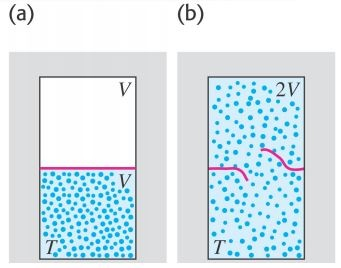
\includegraphics[width=\textwidth]{Entropy1.jpg}
	\end{subfigure}
	\begin{subfigure}{0.3\textwidth}
		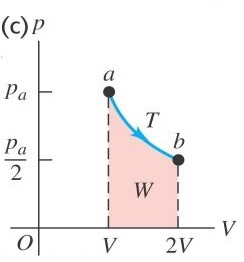
\includegraphics[width=\textwidth]{Entropy2.jpg}
	\end{subfigure}
\end{figure}

\section*{Entropy and the Second Law}
Reversible cycles have a zero net entropy change \\
Irreversible processes always have a positive entropy change (increase in disorder)

New statement of the Second Law: \emph{"No process is possible in which the total entropy decreases, when all systems taking part in the process are included."}

Irreversible processes lead to a loss of opportunity to utilise energy; in a less ordered state, the energy is less available for us to use \\
The universe is continually getting more disordered:
\vspace{-8pt}
\begin{itemize}
	\item Entropy is \emph{the arrow of time}
	\item Ultimate fate of the Universe is heat death
\end{itemize}

\section*{Microscopic Interpretation of Entropy}
Consider N coins:\\
If all N coins are heads, the system is totally ordered \\
The most likely macroscopic state is healf heads and half tails -- there are many possible microscopic states, but little is known about the state of individual coins $\rightarrow$ the system is maximally disordered, and has the most entropy \\
The same arguments can be applied to molecules in a has -- macroscopic p, V, and T vs microscopic position and velocity

\emph{"For any system, the most probable macroscopic state is the one with the greatest number of corresponding microscopic states, which is also the macroscopic state with the greatest disorder and highest entropy."}

\section*{Calculating Entropy From Microscopic States}
For a number, w, of possible microscopic states for a given macroscopic state, the entropy is:
\begin{equation*}
	S = k_{B}\ln{|w|}
\end{equation*}
Increasing the number of states, w, will increase entropy, S \\
Entropy is at a minimum for a single microscopic state:
\begin{equation*}
	w = 1 \implies S = 0, ~ S \nless 0
\end{equation*}
It is more common to calculate $\Delta$S:
\begin{gather*}
	{\Delta}S = S_{2} - S_{1} = k_{B}\ln{|w_{2}|} - k_{B}\ln{|w_{1}|}
	\implies {\Delta}S = k_{B}\ln{\bigg|\frac{w_{2}}{w_{1}}\bigg|}
\end{gather*}

\section*{Microscopic States \& the Second Law}
The entropy of a system can never decrease -- i.e. the number of possible microscopic states can never spontaneously decrease \\
E.g. free compression --
\vspace{-8pt}
\begin{itemize}
	\item All air particles would move randomly to one side of the room
	\item Not impossible, just very unlikely
	\item Probability $\approx \big(\frac{1}{2}\big)^{40000000000000000000000000000}$
\end{itemize}
This has almost certainly never occurred anywhere \\
For all practical purposes, the Second Law has never been violated.
\end{document}
